%Lab Report
\documentclass[12pt,titlepage, a4paper]{article}
 \usepackage[german]{babel}
 \usepackage[utf8]{inputenc}
 \usepackage{graphicx}
 \usepackage[table,usenames,dvipsnames,hyperref]{xcolor}
 \usepackage{multirow}
 \usepackage{caption}
 \usepackage{subcaption}

\begin{document}

\title{Report\\Projektgruppe Kognitive Robotik}

\author{Münstermann,  Cedrick\\  Krombach, Nicola\\[1cm]
	Autonomous Intelligent Systems\\ \textsc{Universität Bonn}\\}



\maketitle


\section*{Abstract}


\section{Einleitung}

Im Rahmen der Projektgruppe Kognitive Robotik sollten in diesem Jahr die Aufgaben der European Robotics Challenges\footnote{http://www.euroc-project.eu/} bearbeitet werden. 
Die Aufgaben der European Robotics Challenges unterteilen sich dabei in drei Challenges, die wiederum verschiedene Unteraufgaben haben:

\begin{itemize}
 \item Challenge 1: Stationäre Manipulationsroboter in Kooperation mit Menschen (Track 1 \& 2)
 \item Challenge 2: Mobile Manipulationsroboter für die Logistik (Track 1 \& 2)
 \item Challenge 3: Flugroboter für industrielle Inspektion (Track 1 \& 2)
\end{itemize}

blabla mehr zu euroc? \\
Autonome Flugroboter eignen sich aufgrund ihres flexiblen Aufbaus und der Möglichkeit schwer zugängliche Objekte anzufliegen, besonders für die Inspektion und Überwachung von sehr großen industriellen
Anlagen oder Infrastrukturen. Dabei sollen sie autonom agieren, sodass auf die Abhängigkeit von einem Piloten verzichtet werden kann.
Auch für die Inspektion von gefährlichen Umgebungen eignet sich ein autonomer Flugroboter.

Unsere Gruppe befasste sich mit dem ersten Track der dritten Challenge, bei welchem die Lokalisierung des MAV und die 3D-Rekonstruktion der Umgebung mit Hilfe von Stereo-Bildern
im Vordergrund stand.



\section{Aufgabenstellung} 
In dem ersten Track von Challenge 3 geht es vorrangig um die Verarbeitung von visuellen Informationen, um die Pose des MAV zu schätzen und schließlich eine Karte von der Umgebung aufzubauen.



\subsection{Task 1 - Visuelle Lokalisierung}
In der ersten Aufgabe ging es darum aus Stereobildern eine 6D-Pose zu schätzen. Dazu wurden realistische Datensätze mit unterschiedlichen Schwierigkeiten zur Verfügung gestellt.
Ausschließlich anhand von diesen Datensätzen sollte nun die Lokalisierung erfolgen. Für die Evaluation war sowohl die lokale Genauigkeit als auch die Echtzeitfähigkeit der Berechnung entscheidend.
Eine \"Ubersicht der Evaluierungskriterien und Punktevergabe findet sich in \cite{eurocannex}.
Neben den Kamerabildern wurden zudem entsprechende Kalibrierungen des Kamerasystems und der IMU zur Verfügung gestellt. 
Für die Berechnung der visuellen Odometrie wurden zunächst zwei bereits in ROS verfügbare Verfahren getestet:\\
Das Paket Semi-direct Monocular Visual Odometry (SVO)\cite{EPFL-CONF-199740} und das Paket LIBVISO2 \cite{Geiger11}.
In ersten Experimenten stellte sich das LIBVISO2 als besser geeignet heraus, und zudem erlaubt es die Verwendung von Stereokameras für die visuelle Odometrie, 
im Gegensatz zu SVO, welches ein monokulares Verfahren ist.
Als Kamerakalibrierung wurde die bereitgestellte Kalibrierung mittels Aprilboard verwendet.
Da die Darstellung der Pose in IMU-Koordinaten erfolgen muss, rechnen wir die Pose mittels einer statischen Transformation aus der Kalibrierung von Kamerakoordinaten in IMU-Koordinaten um.
Die sich dadurch ergebende Transformationskette lautet:\\

$  map \rightarrow imu \rightarrow cam0 $\\

Da keine Groundtruth zur Verfügung gestellt wird, konnte man letztlich nur über die Online-Evaluation herausfinden, wie genau die berechnete Pose ist und wie hoch der relative Fehler ist.
Mit den Default-Werten von LIBVISO2 erhielten wir zu Beginn 4 Punkte bei der einfachsten Schwierigkeit. 
Davon 3 Punkte in der Genauigkeit mit einem mittleren relativen Translationsfehler von 2.6\% und 1 Punkt in der Laufzeit mit 105ms.
Die Laufzeit konnten wir mit dem Setzen des Compiler-Flags DCMAKE\_BUILD\_TYPE auf Release auf 39ms reduzieren, und erhielten so 3 Punkte in der Laufzeit.
Für die Erhöhung der Genauigkeit passten wir die Parameter von LIBVISO2 an die unterschiedlichen Schwierigkeiten an. 
So erhöhten wir den Parameter match\_radius von 100 auf 200 und die RANSAC-Iterationen von 150 auf 160.
Damit konnten wir den Fehler von 2.6\% auf 1.0\% reduzieren, und erhalten damit volle Punktzahl in der Genauigkeit.
Ein Beispiel einer solchen Evaluation ist in Abbildung~\ref{fig:evat1} zu sehen. Dort schneiden wir in der Genauigkeit sehr gut ab, mit einem gemittelten relativen Translationsfehler 
von 1\% erhalten wir für die Genauigkeit volle Punktzahl. Auch in der Laufzeit sind wir mit 40ms verhältnismäßig gut. Für die volle Punktzahl benötigt man eine Laufzeit kleiner 20ms.
Auch in der zweiten Schwierigkeitsstufe erhalten wir mit 8 von 10 möglichen Punkten ein gutes Ergebnis für die berechnete Odometrie. In der schwierigsten Stufe hat die visuelle Odometrie
jedoch einige Probleme die korrekte Pose zu schätzen, was durch die schlechteren Belichtungsverhältnisse und merkmalsärmere Umgebung zu erlären ist.
Wie in Abbildung~\ref{fig:evat3} zu sehen, driften wir vor allem in x- und y-Richtung stark.


\begin{figure}[h!]
 \centering
  \begin{subfigure}[b]{0.49\textwidth}
 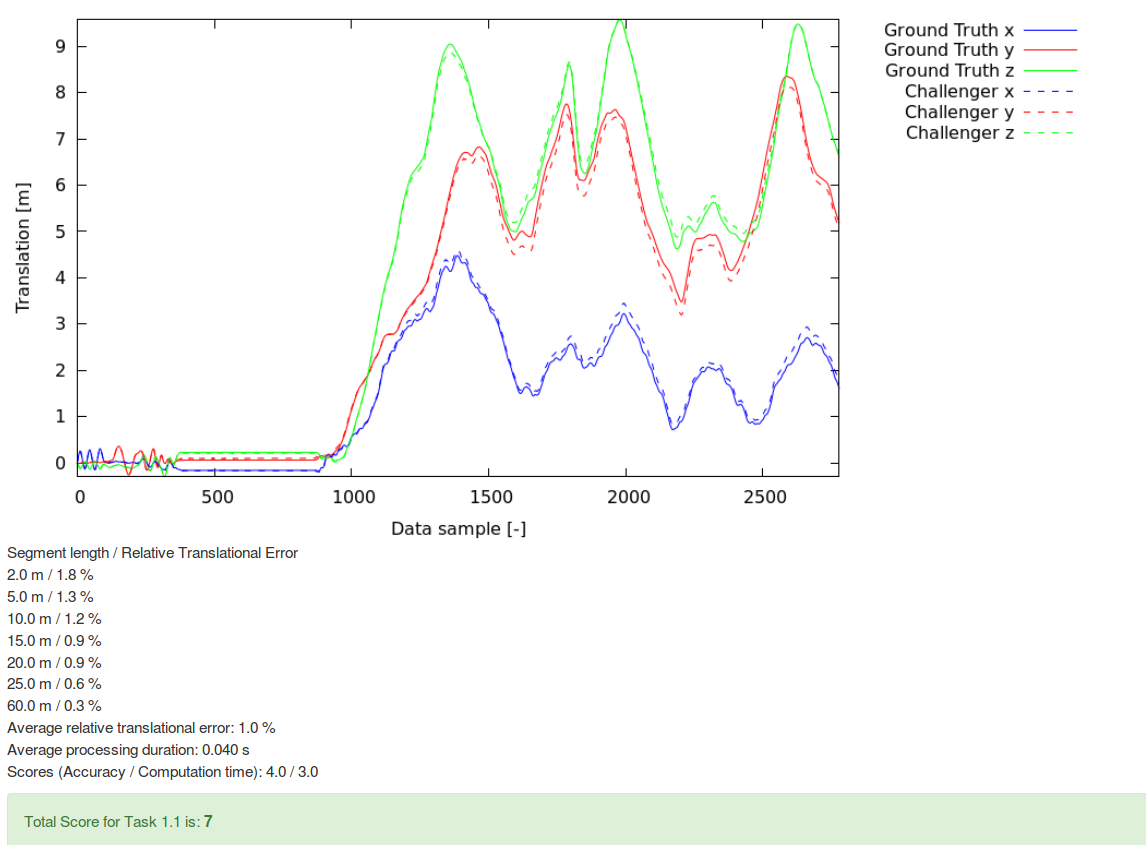
\includegraphics[width=\textwidth]{./Screens/t1_opt2_april.png}\caption{Task 1.1}\label{fig:evat1}  \end{subfigure}
  \begin{subfigure}[b]{0.49\textwidth}
 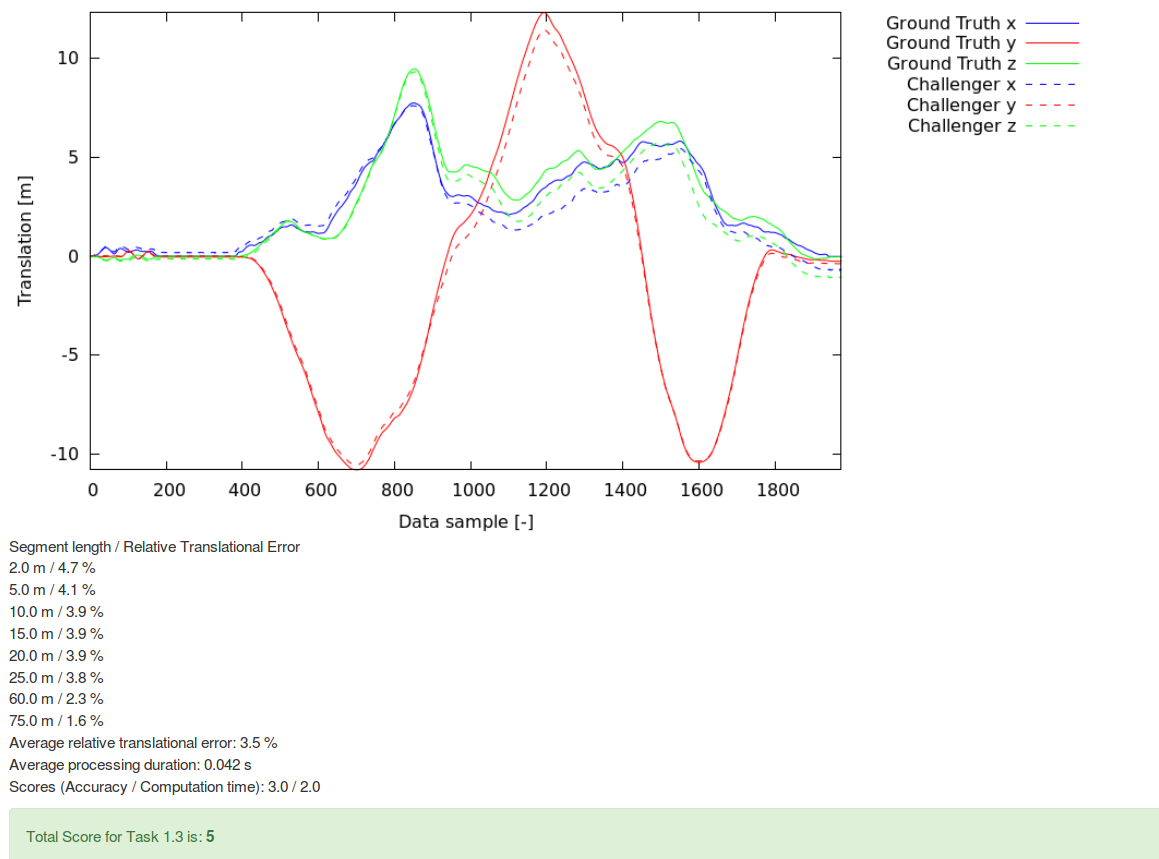
\includegraphics[width=\textwidth]{./Screens/t1_3.png}\caption{Task 1.3}\label{fig:evat3}
 \end{subfigure}
 \caption{Ergebnis der Online-Evaluation zu Task 1.1 und 1.3 mit 7 von 8 (bzw 5 von 8) möglichen Punkten} \label{fig:eva} 
\end{figure}

\begin{table}
\colorlet{tablerowcolor}{green!10.0} 
\centering
\begin{tabular}{c|c|c}
Task & Bewertungsintervall & Punkte\\
\hline
\multirow{5}{*}{1.1 Genauigkeit e} & e \textgreater 20\% & 0 \\
 & e \textless 20\% & 1\\  
  & e \textless 10\% & 2\\
   & e \textless 4\% & 3\\
 &\cellcolor{green!10.0} e \textless 2\% & \cellcolor{green!10.0}4\\
\hline
\multirow{5}{*}{1.1 Laufzeit t} & t \textgreater 200ms & 0 \\
 & t \textless 200ms & 1\\  
  & t \textless 100ms & 2\\
  & \cellcolor{green!10.0}t \textless 40ms &\cellcolor{green!10.0} 3\\
 & t \textless 20ms & 4\\
\hline
\end{tabular}\\
\vspace{10mm}
\caption{Bewertungssystem von EuRoC für Challenge 3 Task 1.1, grün hervorgehoben sind die erziehlten Ergebnisse}
\label{table:scoringt1}
\end{table}
				
\subsection{Task 2 - Mapping}
In der zweiten Teilaufgabe, der dritten Challenge, sollte eine 3D-Karte mit Hilfe des Octomap-Frameworks von Hornung et al. aus Stereobildpaaren und einer jeweils zugehörigen 6D-Pose erstellt werden. Die generierte Karte konnte online überprüft werden. Bewertet wurde anhand des Matthew-Correlation-Coefficient und der Laufzeit. Der Matthew-Correlation-Coefficient nutz das Verhätnis zwischen den als false-free, false-occupied, true-free und true-occupied klassifizierten Voxeln.
Um dieses Problem zu lösen haben wir uns für das elas-Framework von Geiger entschieden um dichte Punktwolken zu generieren.
Die Installation von elas erwies sich aufwendiger als angenommen, da es ROS-Hydro und catkin noch nicht direkt unterstützt. Damit elas unsere Stereobilder gut verarbeiten konnte, mussten diese zunächst noch rektifiziert werden. Mit Hilfe von OpenCV und der gegebenen Kamerakalibrierung die wir schon im ersten Teil in ein OpenCV-konformes Format umgewandelt hatten, war dieser Schritt schnell getan. Was noch fehlte war eine Spezifizierung der Transformationskette vom map-Frame in den Kamera-Frame. Nach Betrachtung der Posen-Nachricht die wir vom Server geliefert bekamen, wussten wir, dass die Pose im IMU-Frame war. Zusätzlich zu den rektifizierten Bildern und der Pose musste nun also auch noch ein Transformation von map auf IMU verfügbar gemacht werden. Die statische Transformation von der IMU zu der Kamera war auch schon aus dem ersten Teil bekannt. Da nun alle Anforderungen der beiden benutzen Frameworks erfüllt waren, konnte die erste Karte erstellt werden. Diese sah auch schon ganz gut aus und stimmte größtenteils mit der von uns handgezeichneten Karte überein. Leider gab es nur wenig Punkte für die Karte. Zwei Punkte für die Akkuratesse und nur Null für die Laufzeit. Um die Laufzeit zu verbessern, beschlossen wir einige Frames zu überspringen. Zunächst war es aber wichtiger die Genauigkeit der Karte zu steigern. Die generierte Voxel-Karte hatte relativ dicke Wände und wir waren uns unsicher inwiefern dies mit in die Bewertung aufgenommen wurde. Als erstes sollten die Wände also dünner werden. Bei Betrachtung der Punktwolke fiel auf, dass an den Rändern dieser keilförmige Falschmessungen in den umliegenden Raum gingen. Um dieses Problem anzugehen bestand ein erster Lösungsansatz einen Filter zu implementieren der auf dem Disparitätsbild ein einem Box-Kernel nach den Minimum und dem Maximum zu suchen und falls die Differenz der beiden über einem Schwellwert lag, den ganzen betrachteten Ausschnitt zu verwerfen. Im Falle von elas auf -10 zu setzen. Leider führte dies nicht zur Eleminierung der Falschmessungen. Siehe Abbildung 2.

\begin{figure}[h!]
	\centering{}
	\begin{subfigure}[h]{0.45\textwidth}
		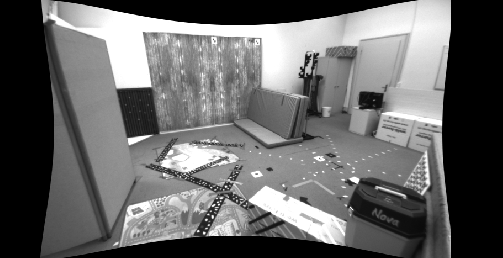
\includegraphics[width=\textwidth]{./jumpEdge/camera.png}
		\caption{after morphing with free space}
	\end{subfigure}\\
	\begin{subfigure}[h]{0.45\textwidth}
		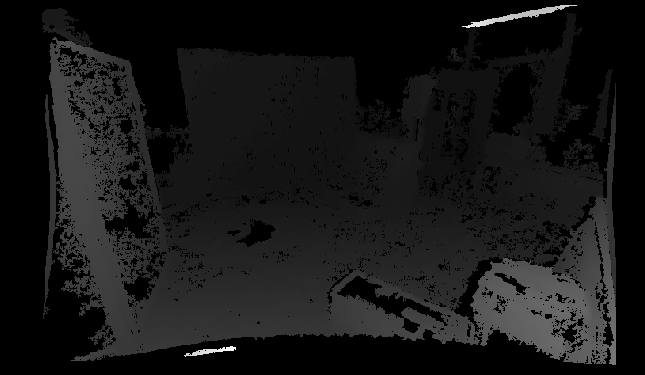
\includegraphics[width=\textwidth]{./jumpEdge/je_off_disparity.png}
		\caption{min-max off}
	\end{subfigure}
	\begin{subfigure}[h]{0.45\textwidth}
		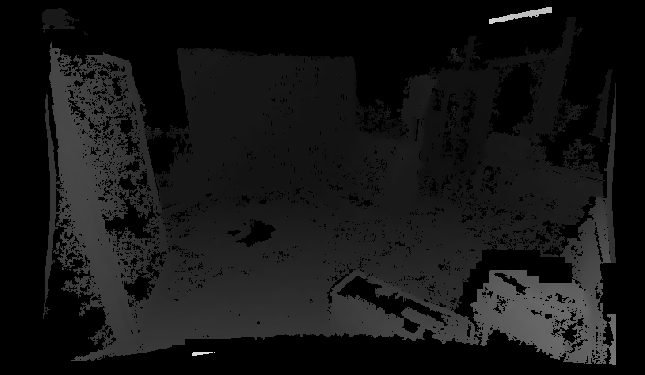
\includegraphics[width=\textwidth]{./jumpEdge/je_on_disparity.png}
		\caption{min-max on}
	\end{subfigure}
	\begin{subfigure}[h]{0.45\textwidth}
		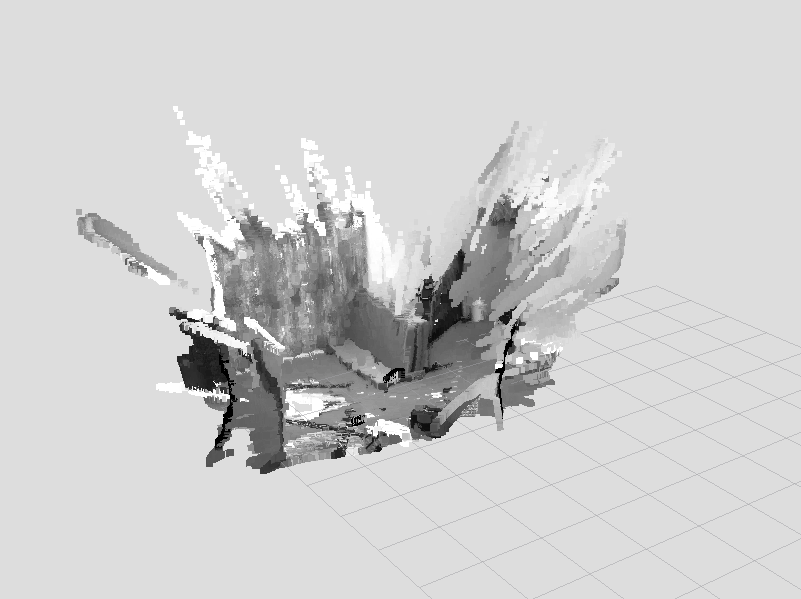
\includegraphics[width=\textwidth]{./jumpEdge/je_off_pointcloud.png}
		\caption{min-max off}
	\end{subfigure}
	\begin{subfigure}[h]{0.45\textwidth}
		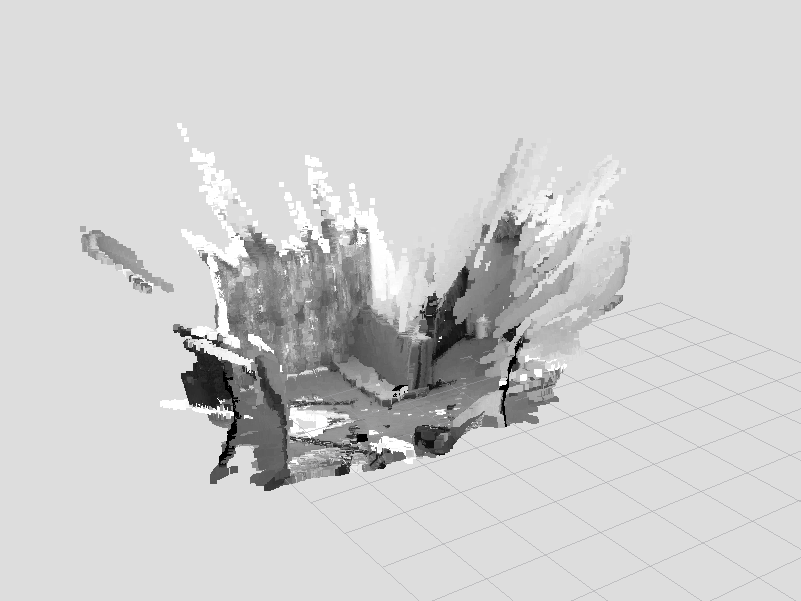
\includegraphics[width=\textwidth]{./jumpEdge/je_on_pointcloud.png}
		\caption{min-max on}
	\end{subfigure}	
 \caption{Pipeline}
\end{figure}

Eine weitere Idee um die Wände auszudünnen und Falschmessungen zu eliminieren, war die generierte Octomap zu prunen nachdem der Occcupancy-Threshold erhöht wurde. Dies führte dann auch zu einer sichtabaren Veränderung in der Map. Die Wände wurden etwas dünner und occupied-Space wurde an manchen Stellen zu unkown- oder free-Space. Auf die finale Bewertung der Map hatte dies jedoch nur minimale Auswirkungen. Auch Parameteranpassungen in elas vorallem die Gap-Interpolation hatten wenig sichtbare Auswirkungen auf das Resultat. Die Gap-Interpolation führte dazu, dass es im Disparitätsbild sehr harte Übergänge in den interpolierten Bereichen auftraten. Um dies zu verhindern filterten wir das Original-Disparitätsbild mit einem Gauss-Filter um glatte Ränder um die Lücken zu bekommen. Dannach interpolierten wir und kopierten die so weich interpolierten Lücken zurück in das Original-Disparitätsbild, um die interessanten Feautures zu behalten aber keine komischen Effekte durch die Gap-Interpolation zu bekommen. Dieser Filter führte nur zu einer minimalen Verbesserung und wurde deswegen wieder verworfen.

Um nun voran zu kommen entschlossen wir uns eine e-mail an den Support zu schreiben um nachzufragen wo genau unser Problem lag.
Zwischenzeitlich hatten wir auch die Vermutung, dass unsere generierte Karte im falschen Koordinatensystem lag und es deshalb zu der mittelmäßigen Bewertung kam.
Wie sich dann durch die e-mail herausstellte waren jedoch weder die dicken Wände noch das Koordinatensystem unser Hauptproblem. Das Bewertungssystem wertete auch unkown-Space der free sein sollte also false-occupied. Unser Problem war, dass wir zu viel unknown-Space in der Nähe der Decke und den Wände hatten. Siehe Abbildung 3.

\begin{table}
\colorlet{tablerowcolor}{green!10.0} 
\centering
\begin{tabular}{c|c|c}
Task & Bewertungsintervall & Punkte\\
\hline
\multirow{5}{210pt}{2.1 Fehler gemessen an Matthews Correlation Coefficient s} & 0 \textless s \textless 0.4 & 0 \\
 & 0.4 \textless  s \textless 0.6 & 1\\  
  & 0.6 \textless  s \textless 0.8 & 2\\
 & \cellcolor{green!10.0}0.8 \textless  s \textless 0.9 &\cellcolor{green!10.0} 3\\
 & 0.9 \textless  s \textless 1.0 & 4\\
\hline
\multirow{5}{210pt}{2.1 Laufzeit t} & t \textgreater $t_{max}$ & 0 \\
 & t \textless $t_{max}$ & 1\\  
  &\cellcolor{green!10.0} t \textless $0.5 t_{max}$ &\cellcolor{green!10.0} 2\\
  & t \textless $0.2 t_{max}$ & 3\\
 & t \textless $0.1 t_{max}$ & 4\\
\hline
\end{tabular}\\
\vspace{10mm}
\caption{Bewertungssystem von EuRoC für Challenge 3 Task 2.1, grün hervorgehoben sind die erziehlten Ergebnisse}
\label{table:scoringt2}
\end{table}

Nun musste also der Freespace immer dann expandiert werden, wenn ein als free klassifizierter Voxel einen Nachbarn hatte, der als unknown klassifiziert war. Aufgrund der Speicherung der Karte in einem Octree sind Voxel die unknown sind nicht explizit in der Datenstruktur gespeichert. Die Expansion des Free-Space führte schließlich auch zu einer deutlichen Verbesserung in der Bewertung. Durch verschiedene Testläufe fanden wir heraus, dass die 4-malige Expansion des Free-Space zu dem besten Ergebnis führten. Noch besser wurde es wenn die fertige Karte davor noch mit einem leicht angepassten Occupancy-Threshold (von 0.7 auf 0.75) geprunt wurde. Siehe Abbildung 4. Es sind jedoch nach wie vor einige fals-occupied übrig und als nächster Schritt wäre es möglich occupied Voxel die weniger als 4 Nachbarn haben die occupied sind auf free zu setzen.

\begin{figure}[h!]
	\centering
	\begin{subfigure}[h]{0.45\textwidth}
		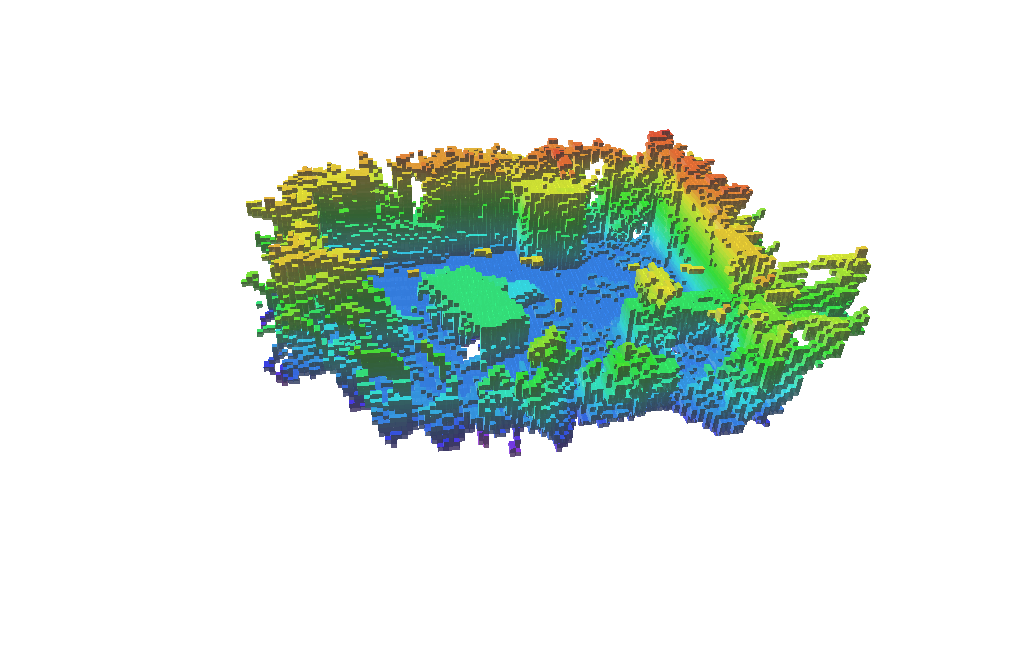
\includegraphics[width=\textwidth]{./maps/beforePrune.png}
		\caption{before pruning}
	\end{subfigure}
	\begin{subfigure}[h]{0.45\textwidth}
		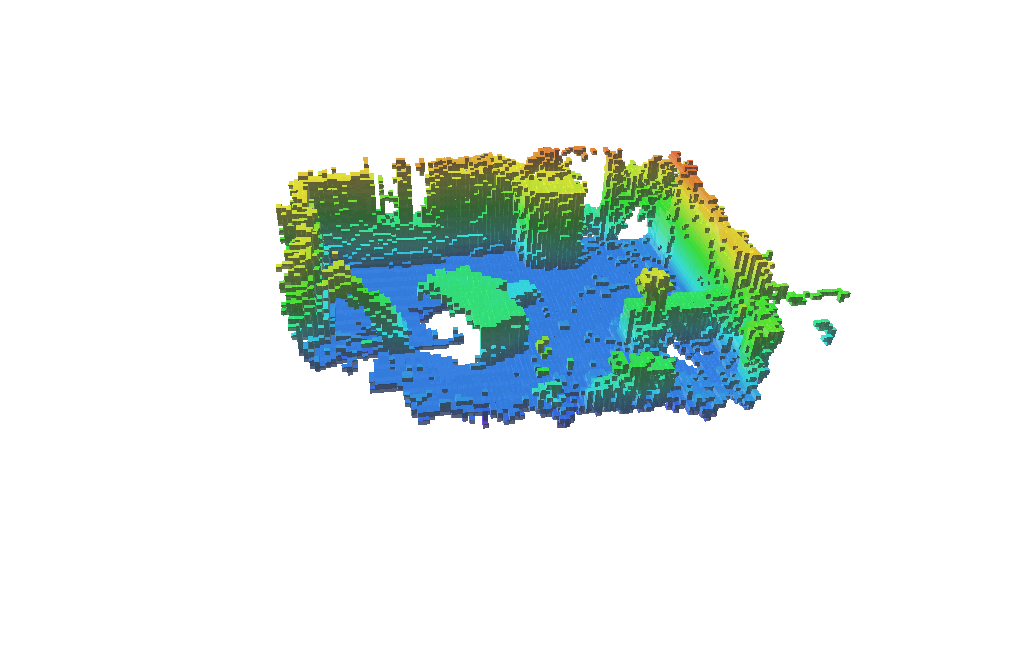
\includegraphics[width=\textwidth]{./maps/beforeMorph.png}
		\caption{after pruning}
	\end{subfigure}\\
	\begin{subfigure}[h]{0.45\textwidth}
		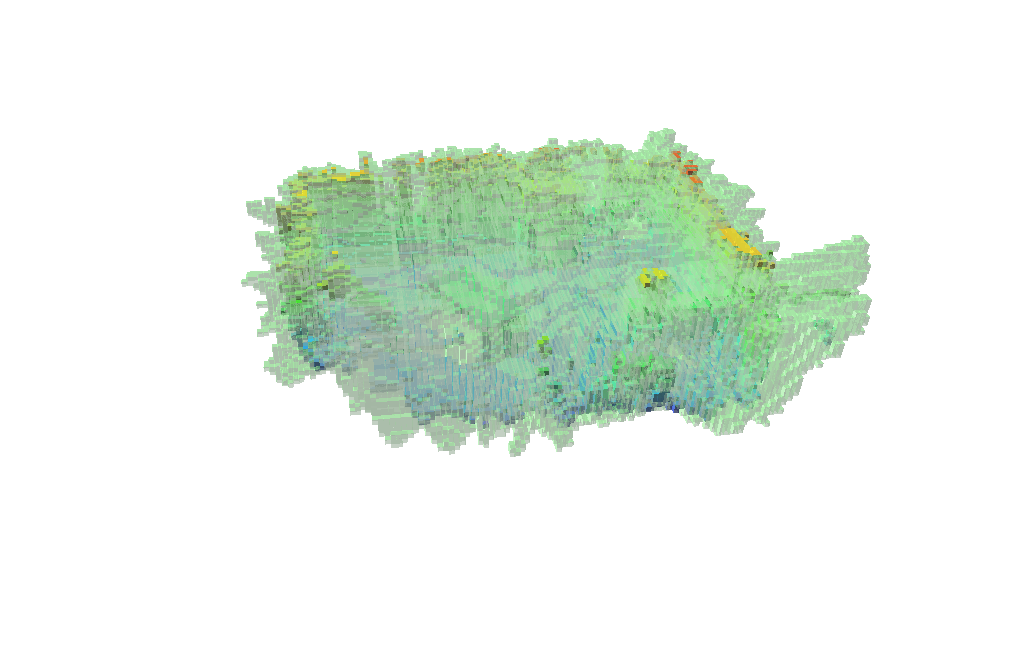
\includegraphics[width=\textwidth]{./maps/beforeMorph_free.png}
		\caption{before morphing with free space}
	\end{subfigure}
	\begin{subfigure}[h]{0.45\textwidth}
		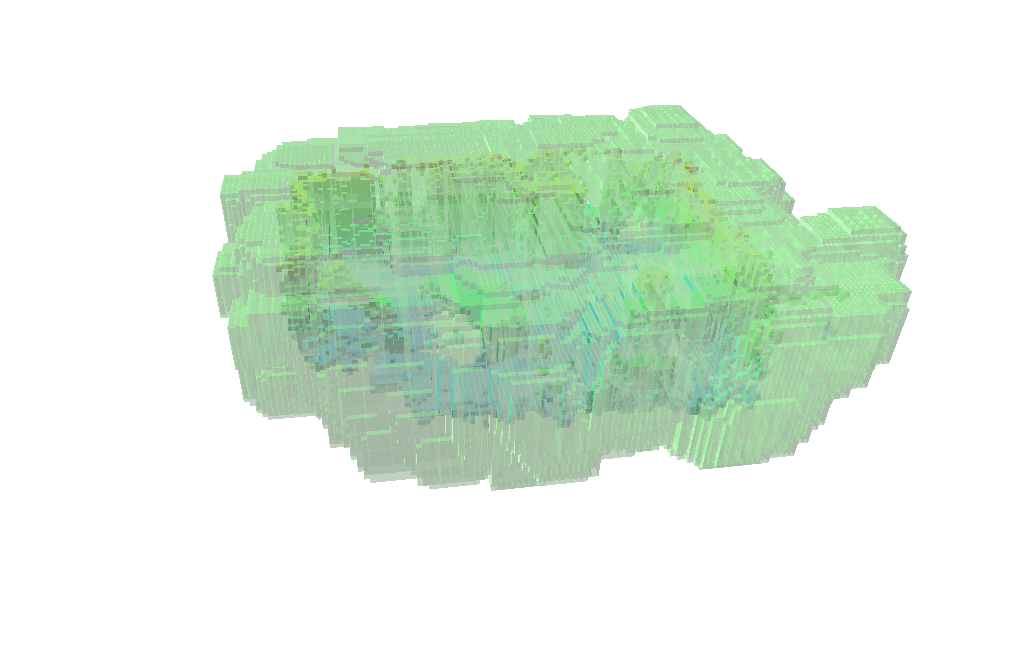
\includegraphics[width=\textwidth]{./maps/afterMorph_free.png}
		\caption{after morphing with free space}
	\end{subfigure}
 \caption{Pipeline}
\end{figure}

\begin{figure}[h!]
 \centering
 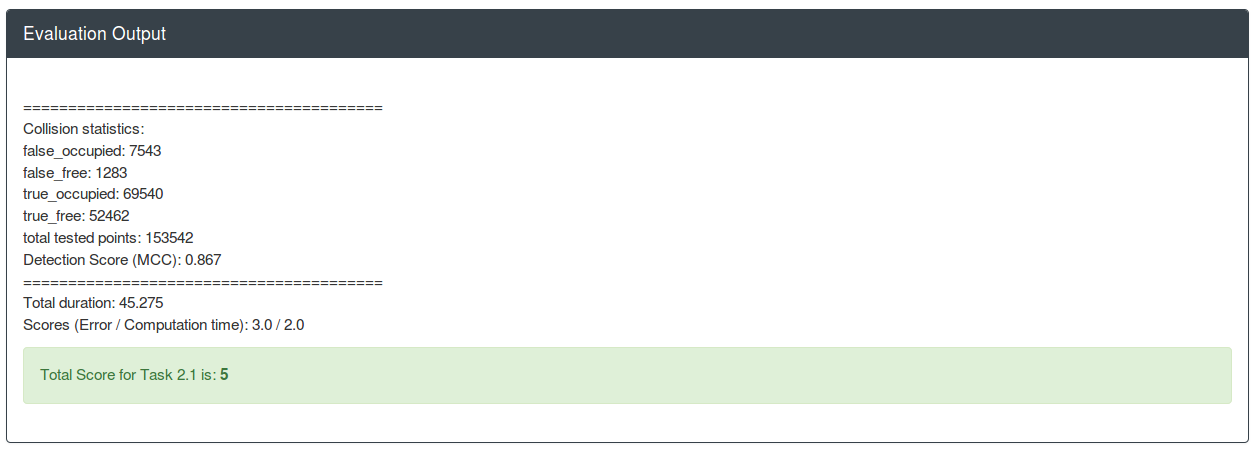
\includegraphics[width=0.5\textwidth]{./Screens/evaltask2.png}
 \caption{Resultat}
\end{figure}

\section{Zusammenfassung}
  \bibliography{lit.bib}
  \bibliographystyle{alpha}
\end{document}
